\documentclass[oneside,a4paper,12pt]{book}
\usepackage{amsmath,amssymb,amsfonts,amsthm}
\usepackage{paralist}
\usepackage{breqn,xy}
\usepackage{array}
\usepackage{longtable}
\usepackage{tikz}
\usetikzlibrary{shapes.geometric,arrows}
\usepackage{subfigure}
\usepackage{graphics}
\usepackage{indentfirst}
\usepackage[shortlabels]{enumitem}
\usepackage{titlesec}
\usepackage{indentfirst}
\usepackage{multicol}
\usepackage[hidelinks=true,bookmarksdepth=3]{hyperref}
\usepackage{xcolor,colortbl}
\usepackage[a4paper, left=3.5cm, right=3.5cm]{geometry}
\usepackage{xepersian}
\settextfont[Scale=1]{XB Niloofar}
\setdigitfont{Yas}
%\newcolumntype{L}{>{\lr\bgroup}l<{\egroup}}
\begin{document}
	
	
	\pagenumbering{arabic}
	\thispagestyle{empty}
		\begin{center}
			\vspace*{4cm}
		\Huge{		\textbf{به نام خدا} \\}
		\Huge{		دانشکده ریاضی و کامپیوتر خوانسار \\}\vspace{1cm}
		\Large{		عنوان پروژه: \\\textbf{تحلیل و طراحی سامانه هوشمند کنترل تردد وسایل نقلیه(ساهک)}\\}\vspace{1cm}
		استاد:\\ \textbf{دکتر فضیلت حججی}\\ \vspace{1cm}
		تهیه کنندگان:\\
		\textbf{عرفان ریاحی، علی کشوری، محمدمهدی هاشمی} \\ \vspace{1cm}
		سرگروه:\\ \textbf{عرفان ریاحی}\\\vspace{1cm}
		پاییز 1399
	\end{center}
	\tableofcontents
	\listoftables
	\listoffigures
	
	\chapter{\rl{مقدمه}}
	در این فصل به تبیین نیازمندی‌های نرم افزار پرداخته‌ایم که در قالب استاندارد \lr{IEEE Std 830-1998} بیان شده است. سامانه هوشمند كنترل تردد افراد و وسايل نقليه (ساهك) باید وظایف نگهبانی و احراز هویت افراد، خودروها و نظارت بر تردد افراد و وسایل نقلیه را انجام دهد.
	\section{\rl{هدف}}
	هدف از سند نیازمندی‌ها، تشریح و تحلیل نیازمندی‌های نرم‌افزار است به گونه‌ای که با بیان آنچه کاربران از سیستم
	انتظار دارند به فرایند توسعه کمک کند. ایجاد یک درک متقابل از پروژه برای توسعه‌دهندگان و کاربران سیستم، تخمین زمان و هزینه توسعه سیستم، تسهیل انتقال سیستم به کاربران یا توسعه‌دهندگان دیگر و کاهش موانع موجود برای توسعه نرم‌افزار از جمله انتظاراتی هستند که امیدواریم این سند آن ها را برآورده سازد.\\
	مخاطبان این سند توسعه‌دهندگان، مهندسین نرم‌افزار و مدیران و صاحبان پروژه هستند.
	
	\section{\rl{دامنه}}
	ساهک، مخفف سامانه هوشمند کنترل تردد افراد و وسایل نقلیه می‌باشد.
	به‌طور کلی این سامانه باید وظایف نگهبانی و احراز هویت افراد، خودروها و نظارت بر تردد افراد و وسایل نقلیه را انجام دهد. برنامه مورد نظر باید نیاز به نیروی انسانی را به حداقل برساند و با کمترین تغییرات در سیستم موجود فعلی، طراحی شود.
	
	\section{\rl{تعاریف، سرنام ها و کوته نوشت ها}}
	\noindent
	\textbf{هيئت:}
	کاربران این سیستم افراد عضو، غیرعضو، ادمین و مهمان هستند، ادمین میتواند لیست تمامی کاربران را مشاهده کند و درصورت نیاز تغییر دهد.\\
	
	\noindent
	\textbf{منطقه‌سبز:} 
	میزان دسترسی هر کاربر و یا گروه کاربران باید مشخص شود و توسط ادمین قابل مشاهده و تغییر باشد. افراد به برخی ساختمانها و حتی برخی محلهای خاص در آن ساختمان می توانند دسترسی داشته باشند و فقط در محلهای مشخصی می توانند خودروی خود را پارک کنند. در غیر اینصورت جریمه میشوند.\\
	
	\noindent
	\textbf{جذب حداكثری:} 
	عضویت کاربران در سیستم برای ورود و خروج به همراه تمدید عضویت.\\
	
	\noindent
	\textbf{كارنامه:}
	صفحه شخصی کاربران به همراه امکان مشاهده گزارش ورود و خروج خود و خودروهایشان به همراه وضعیت عضویت آنان.همچنین ادمین سیستم باید بتواند در پنل خود، آمار ورود و خروج افراد و محل پارک ماشین هایشان را در طول روزهای گذشته مشاهده کند.\\
	
	\noindent
	\textbf{راهنما:}
	پارکینگ هوشمند و راهنمایی کاربران برای پیدا کردن محل پارک در نظر گرفته شده برای آنان.\\
	
	\noindent
	\textbf{مديريت خطا:}
	جریمه خودروهایی که از محدوده تعیین شده و مجوز گرفته شده تجاوز کرده باشند.\\
	
	\noindent
	\textbf{كاروانسرا:}
	امکان تعریف و نظارت بر تردد انواع وسایل نقلیه مثل خودرو شخصی، موتور، اتوبوس، آژانس و جرثقیل.\\
	
	\noindent
	\textbf{باب الرحمة:}
	اتوماسیون دربهای ساختمانها، گیتهای خوابگاه، درهای ورود به محوطه دانشگاه\\
	
	\noindent
	\textbf{چشم عقاب:}
	ردیابی وسایل نقلیه.\\
	
	\noindent
	\textbf{امداد:}
	مدیریت بحران و ارسال درخواست کمک در صورت وقوع اتفاقات مختلف مثل تصادف.\\
	
	\noindent
	\textbf{يار دوازدهم:}
	کمک به نگهبانان در صحت سنجی محل پارک خودروهای پارک شده.
	
	\section{\rl{مراجع}}
	مهندسی نرم‌افزار شی گرا، یک متدولوژی چابک یکنواخت، جلد اول، کونگ- دیوید سی، ترجمه: دکتر بهمن زمانی و
	دکتر افسانه فاطمی، انتشارات دانشگاه اصفهان، چاپ بهار .۱
	۱
	\section{\rl{طرح کلی}}
	در ادامه به شرح و تفصیل واسط‌ها شامل واسط‌های سیستم، کاربر، سخت‌افزار و نرم‌افزار، ارتباطی، حافظه، عملیات و نیازمندیهای سازگاری با محیط نصب می پردازیم، سپس مشخصات کارکرد محصول و مشخصات کاربرانی که با محصول کار میکنند را توضیح می دهیم و در ادامه به بررسی قیود، محدودیت ها و مفروضات پروژه میپردازیم. در آخر هم با بررسی نیازمندی‌ها به تفصیل درباره نیازمندی‌های واسط خارجی و کارکردی و کارایی توضیح میدهیم.
	
	
	
	\chapter{\rl{شرح کلی}}
	ساهک برای تسهیل فرایند‌های موجود در سیستم کنترل پارکینگ  شامل بررسی موقعیت خودرو و احراز هویت و کنترل فضاهای پارک خودرو و  تأمین امنیت کاربران و خودروها و تشخیص تخلفات و جریمه‌ی خودکار افراد متخلف می‌باشد.
	\section{\rl{چشم انداز محصول}}
	
	\subsection{\rl{واسط‌های سیستم}}
	ساهک برای گزارش جرایم با پلیس، آتش سوزی و اطفای حریق با آتش نشانی و آسیب دیدگی های فردی با اورژانس و حلال احمر ارتباط برقرار میکند.
	
	\subsection{\rl{واسط‌های کاربر}}
	ساهک از طریق وب اپلیکیشن و اپلیکیشن های اندروید و \lr{IOS} و مانیتور‎های تعبیه شده در ورودی ها با مخاطب ارتباط برقرار می‌کند.
	
	
	\subsection{\rl{واسط های سخت افزاری}}
	\begin{itemize}[label = --]
		\item\noindent
		برای شناسایی خودرو براساس پلاک از دوربین مخصوص استفاده می‌کنیم و این دوربین ها باید قابلیت دید در شب داشته باشند.
		\item\noindent
		در ابتدای ورودی ها از دوربین‌های ثابت و در محوطه‌ی پارکینگ از دوربین‌های گردان استفاده می‌کنیم.
		\item\noindent
		ساهک از مانیتور برای نشان دادن وضعیت پارکینگ استفاده می‌کند.
		\item\noindent
		از سیستم اعلام و اطفای حریق استفاده می‌کند که برای شناسایی و اطفا حریق مورد استفاده قرار می‌گیرد.
		\item\noindent
		از سنسور مادون قرمز برای اعلام وضعیت محل پارک موردنظر استفاده می‌کنیم.
		
		\item\noindent
		برای مدیریت و کنترل دوربین های مداربسته از سیستم های کنترلی استفاده می‌کنیم که این سیستم شامل دستگاه های ذخیره سازی، دستگاه های کنترل کننده\lr{(DVI)} می‌باشد.
		\item\noindent
		از چراغ های مخصوص برای راهنمایی کاربران استفاده می‌شود.
		\item\noindent
		از کارت های مخصوص برای ثبت ورود و خروج استفاده می‌شود که شامل دو کارت می‌شود: 1)ویژه مهمانان 2)کارت پرسنلی و دانشجویی و همچنین از دستگاه‌ کارت خوان برای شناسایی کارت‌ها استفاده می‌کنیم.
		
		\item\noindent
		گیت ورود و خروج افراد و ماشین
	\end{itemize}
	
	\subsection{\rl{واسط های نرم افزاری}}
	ساهک برای پرداخت جریمه از سیستم شاپرک استفاده می‌کند.
	
	\subsection{\rl{واسطه های ارتباطی}}
	کلاینت‌های مختلف ساهک از طریق سرور و شبکه های ارتباطی درونی با هم ارتباط برقرار می‌کنند. این ارتباط با استفاده از اینترنت و اینترانت می‌باشد.
	
	\subsection{\rl{واسطه های حافظه}}
	ساهک برای ذخیره سازی اطلاعات هر دوربین مداربسته ماهانه به یک هارد 1 ترابایتی برای حافظه اصلی و از 5 ترابایت حافظه موقت برای ذخیره سازی اطلاعات کلیه دوربین ها استفاده می‌کند. ساهک برای تهیه‌ی نسخه پشتیبان خود به یک حافظه 50 ترابایتی نیاز دارد.
	
	\subsection{\rl{واسطه های عملیات}}
	\begin{enumerate}[label = --]
		\item\textbf{تغییر در اشیا کسب و کارهای\lr{(Business objects)}سیستم:}
		هنگام اعمال تغییرات سیستم پیغام مرتبط به کاربران را نشان میدهد.
		
		\item\textbf{تعمیرات حین فعالیت سیستم:}
		هنگام اعمال تغییرات، غیرفعال شدن سیستم با نشان دادن پیغام مرتبط به کاربران اطلاع کاربران میرسد.
		
		\item\textbf{پشتیبان گیری:}
		پیشبینی روشی در سیستم پایگاه داده برای پشتیبان گیری
		
	\end{enumerate}
	
	\subsection{\rl{نیازمندی های سازگاری با محیط نصب}}
	\begin{enumerate}[label = --]
		\item\textbf{پایگاه داده پشتیبان:}
		در راستای افزایش امنیت اطلاعات حساس، چندین پایگاه داده پشتیبان پیشبینی شده است.
		\item\textbf{مولد برق پشتیبان:}
		سیستم توزین بار در محل نیاز دارد که حتی در صورت قطع برق فعال باشد. در نتیجه برای
		هر واحد توزین بار، یک مولد برق پشتیبان پیش بینی شده است.
		\item\textbf{سرور پشتیبان:}
		در صورت افزایش بیش حد بار روی سرور اصلی، سرور اصلی نباید غیرفعال شود. در نتیجه
		سرور پشتیبان پیشبینی شده است.
	\end{enumerate}
	
	\section{\rl{کارکرد محصول}}
	ساهک به منظور تسهیل و اتوماسیون فرایندهای کنترل پارکینگ امور زیر را انجام می‌دهد:
	\begin{enumerate}
		\item
		حفاظت و نگهداری از خودروها
		\item
		ارائه کارنامه فعالیتی
		\item
		مدیریت رفت و آمدهای اشخاص ، خودرو ها و ...
		\item
		دریافت بازخورد از کاربران
		\item
		محاسبه و کنترل هزینه‌های پارکینگ
	\end{enumerate}
	
	
	\section{\rl{مشخصات کاربر}}
	کاربران ما شامل دانشجویان، اساتید، پرسنل، مردم، ناظران و پیمانکاران می‌شوند. کاربران برای استفاده از ساهک باید با مفاهیم اولیه کامپیوتر و دستگاه هوشمند آشنایی داشته باشند و برای پرسنل مرتبط با سیستم باید یک جلسه‌ی توجیهی گذاشته شود.
	\section{\rl{قیود}}
	\noindent
	هر نام کاربری فقط یکبار اجازه ورود به سیستم را دارا می‌باشد و ورود مجدد بدون خروج از سیستم امکان پذیر نمی‌باشد.
	
	\noindent
	هر نام کاربری منحصربه‌فرد بوده و قابل استفاده برای اشخاص دیگر نمی‌باشد.
	
	\noindent
	هر نام کاربری برای استفاده از امکانات سیستم نیازمند ثبت نام و خرید اعتبار برای یک بار به صورت اجباری می‌باشد. اعتبار هر نام کاربری پس از دوره مشخص به پایان می‌رسد که کاربر برای ادامه استفاده از سیستم می‌بایست آن را تمدید نماید.
	
	\noindent
	جرائم هر نام کاربری باید به صورت ماهانه پرداخت گردد در غیر این صورت اجازه خروج از سیستم را دارا نمی‌باشد و اعتبار هر کد در صورت عدم پرداخت خاتمه می یابد و و امکان تمدید تا پرداخت جرائم وجود ندارد.
	
	
	\section{مفروضات و وابستگی ها}
	\noindent
	ساهک باید دسترسی به اینترنت و پشتیبان‌گیری شبانه روزی داشته باشد.
	
	\noindent
	ساهک باید به اطلاعات دیتابیس‎های دانشگاه نظیر اطلاعات افراد ، پرسنل ، دانشجوها، کارکنان، خوابگاه‌ها و ساختمان‌ها را داشته باشد. 
	
	\noindent
	ساهک از سیستم دوربین‌های مداربسته موجود و دیگر امکانات دانشگاه پشتیبانی کرده و از آنها استفاده می‎کند.
	
	\noindent
	گزارش‌های ساهک وجهه قانونی داشته و از اعتبار حقوقی برخوردار است.
	
	
	\chapter{نیازمندی های خاص}
	\section{نیازمندی های واسط خارجی}
	\subsection{واسط‌های سیستم}
	\noindent
	ساهک در صورت صلاح دید مسئول مربوطه تخلفات هر شخص ، خودرو یا ... را برای ارگان های قضایی و اجرایی ارسال می‌نماید.
	
	\noindent
	ساهک در صورت وقوع حادثه با ارگان های مربوطه نظیر آتش نشانی یا واحد های امداد و نجات ارتباط برقرار میکند.
	\subsection{واسط‌های کاربر}
	\noindent\textbf{وب اپلیکیشن:} هر کاربر می‌تواند با استفاده از مشخصات خود در سیستم وارد شود و گزارشات مربوط به خود را مشاهده کرده، از وضعیت حساب خود باخبر شود، اعتبار خود را تمدید کرده و یا فعال نماید و همچنین در نظرسنجی های موجود شرکت نماید.\\
	
	\noindent\textbf{اپلیکیشن های همراه:} هر کاربر می‌تواند با نصب اپلیکیشن ساهک به تمامی اطلاعات فوق که در سایت در دسترس است نیز دسترسی داشته باشد.\\
	
	\noindent\textbf{مانیتورهای ارتباطی:} کاربران می‌توانند با استفاده از مانیتورهای ارتباطی تعبیه شده در نقاط مختلف با سیستم در ارتباط بوده و از راهنمایی‌های آنها استفاده نمایند، همچنین ارتباط تعاملی این مانیتور ها با کاربران اجازه بهبود شرایط و آگاهی از اتفاقات را به سیستم می‌دهد.
	
	\subsection{واسط‌های سخت افزاری}
	\noindent\textbf{دوربین‌های مدار بسته:} دوربین‌های مداربسته با استفاده از رهگیری کاربران سیستم همچنین دریافت اطلاعات از محیط و بهره‌گیری از سیستم هوش مصنوعی و پردازش تصویر می‌توانند اتفاقات در حال وقوع را ثبت و ضبط نمایند .
	سنسورهای اعلام و اطفاء حریق: این سنسورهای با استفاده از اطلاعات دریافتی از محیط در صورت وقوع آتش‌سوزی به سیستم مرکزی هشدار داده و همچنین ارگان های مربوطه را خبر می‌کند و در حد توان تلاش می‌کند تا از گسترش آتش جلوگیری کرده و آن را مهار کند.\\
	
	\noindent\textbf{سنسورهای مادون قرمز:} این سنسورها در هر مکان پارک تعبیه شده و قادر است وضعیت محل پارک را مورد ارزیابی قرار دهد، همچنین با ارتباط با سیستم چراغ های راهنما می‌تواند باعث هدایت آسان تر افراد در پارکینگ شود.\\
	
	\noindent\textbf{مانیتور:} با استفاده از این مانیتورها کاربر می‌تواند از اطلاعات نسبی هر پارکینگ با خبر شود و همچنین از آنها برای راهنمایی کاربران نیز استفاده می‌شود این مانیتورهای در قسمت های دیگر نیز با افراد در ارتباط بوده و اطلاعات مورد نیاز را نشان خواهد داد.\\
	
	\noindent\textbf{کارت الکترونیکی:} کارت‌های الکترونیکی کارت‌های دارای چیپستی می‌باشند که اطلاعات هر فرد بر روی آن نوشته می‌شود مانند کارت های دانشجویی یا کارت پرسنلی که پل ارتباط سیستم با کاربران بوده و در محل های بسیاری مورد استفاده قرار می‌گیرد. این کارت ها در ابتدای فعالیت هر شخصی در این سیستم به او داده می‌شود همچنین افراد مهمانی که به صورت موقت از این سیستم استفاده می‌کنند کارت مهمان داده می‌شود که در هنگام خروج باید تحویل داده شود. \\
	
	\noindent\textbf{گیت‌های ورود و خروج:} گیت‌های تعبیه شده در بخش های ورودی هر ساختمان ، درب‌های ورودی و یا هر مکان دیگر که نیازمند ثبت تردد افراد می‌باشد هستند که با کارت‌های الکترونیکی موجود همخوانی داشته و مورد استفاده می‌باشند.
	
	\subsection{واسط‌های نرم‌افزاری}
	در این سیستم ارتباط بین سخت‌افزار و نرم‌افزار وجود دارد که در هر مکان بر اساس استانداردهای تعیین شده از \lr{API}  های موجود و یا زبان مناسب برای برقراری ارتباط با سیستم استفاده می‌شود.
	\subsection{واسط‌های ارتباطی}
	برای برقراری ارتباط بین کلاینت‌ها و سرورها از اینترنت استفاده می‌شود. به منظور ایجاد این قابلیت برای تمام
	کلاینت‌ها، کاربران باید با اینترنت همراه تعبیه شده برای آنها از جمله مودم‌های همراه و اینترنت سیمکارت‌ها، به
	شبکه‌ی اینترنت به صورت شبانه‌روزی دسترسی داشته باشند. همچنین دیگر بخش‌های سیستم می‌توانند با استفاده از اینترانت و بستر شبکه با یکدیگر در ارتباط باشند.
	
	\section{نیازمندی های کارکردی}
	\begin{enumerate}[$ R. 1 $]
		
		\item
		سیستم باید کارت کاربر را خوانده و با تایید اطلاعات اجازه ورود بدهد.
		\item
		سیستم باید در صورت تایید اطلاعات هویتی شماره پلاک خودرو را ثبت کند.
		\item
		سیستم باید لحظه ی ورود و خروج کاربر را ذخیره کند.
		\item
		سیستم باید توانایی تشخیص وضعیت جای پارک را داشته باشد.
		\item
		سیستم باید توانایی ارائه گزارش از وضعیت پارکینگ ها را داشته باشد.
		\item
		سیستم باید توانایی کنترل گیت های ورودی و خروجی را داشته باشد.
		\item
		سیستم باید توانایی رهگیری خودروها را داشته باشد.
		\item
		سیستم باید توانایی راهنمایی کاربران به محل های مورد نظرشان را داشته باشد.
		\item
		سیستم باید توانایی برقراری ارتباط تعاملی با کاربران را داشته باشد.
		\item
		سیستم باید بتواند با استفاده از سیستم های اعلام حریق وقوع آتش سوزی را گزارش دهد.
		\item
		سیستم باید بتواند با استفاده از سیستم های اطفای حریق آتش سوزی را  کنترل نموده یا آن را خاموش نماید.
		\item
		سیستم باید بتواند در صورت وقوع حادثه های اورژانسی به ارگان های مربوطه گزارش دهد.
		\item
		سیستم باید با استفاده از پردازش تصویر نوع حادثه را تشخیص دهد و اقدام لازم را به عمل آورد.
		\item
		سیستم باید در موقع خروج بتواند اطلاعات مربوط به کاربر را با اطلاعات موجود در دیتابیس تطابق دهد و در صورت تطابق اجازه خروج دهد، در صورت عدم تطابق مورد را گزارش دهد و از خروج کاربر ممانعت نماید.
		\item
		سیستم باید بتواند با استفاده از گزارشات موجود رفتار خودرو را تحلیل نموده و نسبت به جریمه نمودن کاربر اقدام نماید.
		\item
		سیستم باید بتواند کاربران دارای جرایم را مورد بررسی قرار داده و اقدامات لازم را برای آنان عمل آورد.
		\item
		سیستم باید توانایی تشخیص هر گروه از کاربران را داشته باشد و اقدامات لازم متناسب با آنها را انجام دهد.
		
		\subitem
		$ R. 17. 1 $		سیستم باید بتواند کاربران مهمان مدیریت نماید.
		\subitem
		$ R. 17. 2 $		سیستم باید از ارائه خدمات به کاربران غیر عضو ممانعت نماید.
		\item	
		سیستم باید بتواند گزارشات موجود را در اپلیکیشن ها ثبت نماید.
		\item
		سیستم باید گزارشات را به صورت دوره ای برای هر کاربر با دسترسی مربوطه ارسال کاربر نماید.
	
	\end{enumerate}
	\section{نیازمندی های کارایی}
	\noindent
	ساهک باید توانایی رهگیری 500 شخص را به طور هم زمان داشته باشد.\\
	\noindent
	ساهک باید بتواند حداکثر وضعیت 30 خودرو را به طور همزمان کنترل کند.	\\
	\noindent
	ساهک باید بتواند در روز حداکثر ورود و خروج 20000 خودرو را کنترل نمیاد.\\
	\noindent
	ساهک باید توانایی کنترل و گزارش‌دهی 15 خوابگاه را داشته باشد. \\
	\noindent
	ساهک باید توانایی کنترل و گزارش‌دهی حداقل 4 پارکینگ را داشته باشد.\\
	\noindent
	ساهک باید توانایی انتقال 10 گیگابایت اطلاعات را در شبکه داخلی خود در لحظه داشته باشد.
	
	\section{قیود طراحی}
	\subsection{زبان برنامه نویسی و توسعه}
	زبان برنامه نویسی برای طراحی این سیستم، سیستم چند زبانه می‌باشد که بر اساس کارکرد متفاوت است.
	\subsection{سرور سیستم}
	سرور مورد استفاده برای ساهک سرور تحت لینوکس است که نیاز های امنیتی مورد نظر را برطرف نماید.
	\subsection{بودجه‌ی مالی}
	بودجه‌ی درنظرگرفته شده برای بخش نرم افزار حداکثر \lr{-n}میلیون تومان می‌باشد.
	\subsection{بودجه‌ی زمانی}
	با توجه به تغییر زیرساخت و عملکرد دانشگاه‌، این نرم‌افزار، باید ظرف مدت حداکثر \lr{-m}ماه آماده شود.
	
	\section{صفت‌های سیستم نرم افزاری}
	\subsection{قابلیت اطمینان}
	ساهک باید در ۹۹درصد مواقع در دسترس باشد.
	\subsection{نرخ خطا}
	\noindent
	ساهک باید حداکثر از هر ۲۰صورت وضعیت، ۱مورد اشکال داشته باشد.
	
	
	\subsection{رعایت استاندارد امنیتی \lr{IEEE STD-1228}}
	جهت تامین امنیت سیستم هنگام توسعه، راه‌اندازی و نگهداری مفاد این استاندارد رعایت شده است.
	
	
	\chapter{مدل دامنه}
	\section{گام جمع آوری اطلاعات دامنه‌ی کاربرد}
	به دلیل شرایط کرونا و نامناسب بودن شرایط محیطی دسترسی به افراد مرتبط ناممکن بوده و تمامی اطلاعات به صورت فرضی و نمادین بوده و همچنین الگوبرداری از نمونه‌های موجود بوده است.
	
	\section{گام طوفان فکری}
	بعد از تحلیل اطلاعات بدست آمده از گام قبل، مباحث مرتبط دسته‌بندی شده‌اند. به دلیل محدودیت زمانی و صلاح دید اعضای گروه تیم ۳ نفرهای تشکیل شد و گام طوفان فکری و دسته بندی طوفان فکری برای هر دسته از اطلاعات به طور جداگانه در هر جلسه‌ی ۱ تا ۲ ساعتی اجرا شد. در انتهای اجرای طوفان فکری و دسته بندی نتایج آن برای هر بخش اطلاعات زمانی برای ترکیب آنها صورت گرفت .

	%\renewcommand{\arraystretch}{2}
	\vspace{6cm}
	\section{گام دسته بندی نتایج طوفان فکری}
	%\begin{table}[b]
	\begin{center}
		\begin{longtable}{|r|l|}
			\hline
			\textbf{فهرست طوفان فکری} & \textbf{نتایج دسته بندی} \\
			\hline
			\hline
			کاربر & \lr{(C) user} \\
			\hline
			نام کاربر & \ \lr{(A) name} \\
			\hline
			شناسه کاربر & \ \lr{(A) id} \\
			\hline
			دسترسی کاربر & \lr{(A) access} \\
			\hline
			خودرو & \lr{(C) vehicle} \\
			\hline
			پلاک خودرو & \lr{(A) plaque} \\
			\hline
			نوع خودرو & \lr{(A) type} \\
			\hline
			رنگ خودرو & \lr{(A) color} \\ 
			\hline
			دسترسی خودرو & \lr{(A) access} \\
			\hline
			کارت هوشمند & \lr{(C) smart card} \\
			\hline
			شماره سریال & \lr{(A) serial} \\
			\hline
			تاریخ اعتبار & \lr{(A) validity date} \\
			\hline
			پارکینگ & \lr{(C) parking} \\
			\hline
			وضعیت & \lr{(A) status} \\
			\hline
			گیت ورود و خروج & \lr{(A) I/O gate} \\
			\hline
			کارتخوان & \lr{(A) cardreader} \\
			\hline
			مانیتور & \lr{(A) monitor} \\
			\hline
			جای پارک & \lr{(C) parking space} \\
			\hline
			وضعیت & \lr{(A) status} \\
			\hline
			نوع & \lr{(A) type} \\
			\hline
			سنسور & \lr{(C) sensor} \\
			\hline
			نوع & \lr{(A) type} \\
			\hline
			مقدار & \lr{(A) value} \\
			\hline
			سیستم گزارش & \lr{(C) report system} \\
			\hline
			نوع & \lr{(A) type} \\
			\hline
			تاریخ & \lr{(A) date} \\
			\hline
			زمان & \lr{(A) time} \\
			\hline
			فرستنده & \lr{(A) sender} \\
			\hline
			توضیحات & \lr{(A) explain} \\
			\hline
			سیستم رهگیری & \lr{(C) tracking system} \\
			\hline
			سوژه & \lr{(A) case} \\
			\hline
			کاربر & \lr{(A) user} \\
			\hline
			دوربین & \lr{(A) camera} \\
			\hline
			دستگاه ذخیره & \lr{(A) Storage device} \\
			\hline
			سیستم ارتباطی & \lr{(C) communication system} \\
			\hline
			کاربر & \lr{(A) user} \\
			\hline
			راهنما & \lr{(A) guide} \\
			\hline
			اطلاعات & \lr{(A) information} \\
			\hline
			مانیتور & \lr{(A) monitor} \\
			\hline
			سیستم مالی & \lr{(C) financial system} \\
			\hline
			کاربر & \lr{(A) user} \\
			\hline
			صورتحساب & \lr{(A) bill} \\
			\hline
			سیستم جریمه & \lr{(C) penalty system} \\
			\hline
			کاربر & \lr{(A) user} \\
			\hline
			تاریخچه & \lr{(A) history} \\
			\hline
			مقدار & \lr{(A) amount} \\
			\hline
			مهلت پرداخت & \lr{(A) payment deadline} \\
			\hline
			وضعیت & \lr{(A) status} \\
			\hline
			
			\caption{دسته بندی نتایج طوفان فکری}
		\end{longtable}	
	\end{center}
	%\end{table}
	\vspace{10cm}
	\begin{figure}
		\begin{center}
			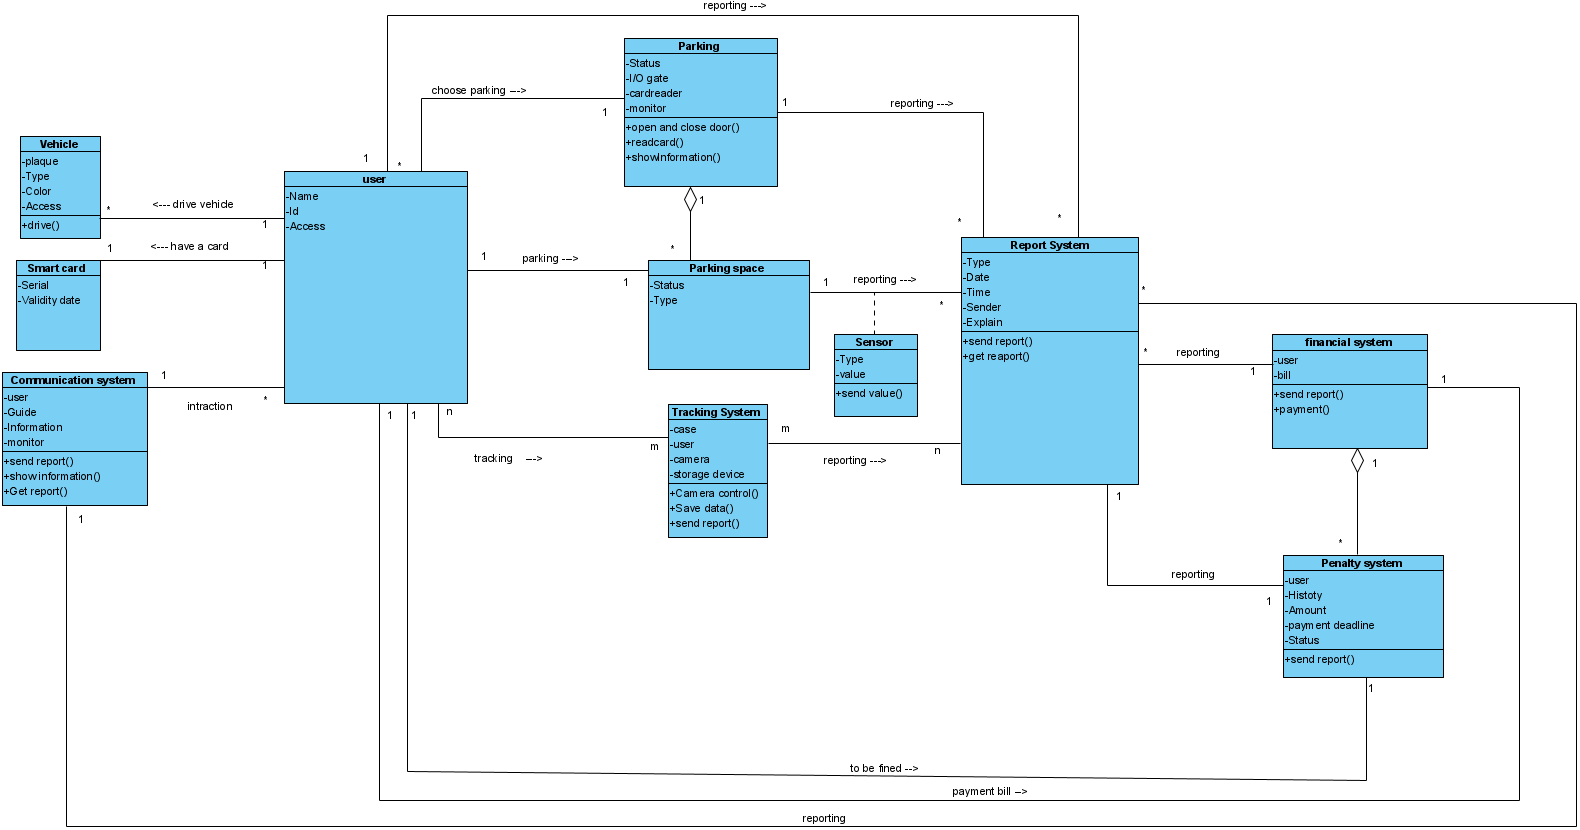
\includegraphics[width=16cm]{DomainModel.png}
			\caption{مدل دامنه سیستم ساهک}
		\end{center}
	\end{figure}
	\section{مرور مدل دامنه}
	در این گام به منظور شناسایی خطاها و اشکالات و اطمینان از کامل بودن، جلسه‌هایی با دیگر اعضای گروه برگزار شد و
	نتایج بدست آمده در گروه قبل برای بار دیگر مورد بحث و تحلیل قرار گرفت. طبق این جلسات کلاس‌های مربوط به
	گزارشات و تعداد محدودی از رابطه‌ها در مدل دامنه تغییر نمود.
	
	\chapter{معماری سیستم}
	طراحی معماری سیستم یک فرایند تصمیم گیری برای تعیین مسیر طراحی سیستم می‌باشد. یک معماری سیستم
	مناسب برای توسعه سیستم چارچوب مشخصی را ایجاد می‌کند و باعث ایجاد زیرساخت قوی در سیستم می‌شود که آن
	را برابر مشکلات احتمالی مقاوم می‌کنند و اعمال تغییرات مورد نیاز را آسان می‌کند.
	
	\section{تعیین اهداف معماری}
	طراحی معماری با هدف ایجاد یک معماری کلی برای سیستم نرم‌افزاری انجام می‌گردد همچنین هدف از طراحی
	معماری نرم افزار افزایش درک و هماهنگی توسعه‌دهندگان و تعامل آسان‌تر با معماری نرم‌‍افزار می‌باشد و افزایش قابلیت
	نگهداری نرم‌افزار و استفاده مجدد و سهولت ایجاد تغییرات نیز در اهداف معماری در نظر گرفته می‌شود.
	
	\section{تعیین نوع سیستم، تعیین واسطه ها و زیرسیستم ها}
	\noindent
	سیستم ساهک تلفیقی از معماری تعاملی، رویداد-رانده و پایگاه داده است. \\
	سیستم درخواست‌ها را از کاربر دریافت و پردازش می‌کند و با تعامل با کاربر موجودیت‌ها را مدیریت (مدیریت پارکینگ) می‌کند. از آنجا که بخشی از درخواست‌ها به صورت تصادفی از بخش سخت‌افزاری سیستم ارسال می‌شود، معماری سیستم با معماری رویداد رانده و معماری پایگاه داده تلفیق شده است.\\
	\noindent
	معماری کلی سیستم از چندین واحد تشکیل شده است که هر کدام بسته به نوع فعالیت خود دارای معماری خاصی است.
	\begin{table}
		\begin{center}
			\begin{tabular}{|p{1cm}|p{5cm}|p{5cm}|}
				\hline
				\textbf{ردیف} & \textbf{واحد} & \textbf{نوع معماری} \\
				\hline
				1 & کنترل مرکزی & رویداد-رانده \\
				\hline
				2 & نظارت & رویداد-رانده \\
				\hline
				3 & مالی & رویداد-رانده \\
				\hline
				4 & ارتباطی & تعاملی \\
				\hline
				5 & گزارش & تعاملی \\
				\hline
				6 & پایگاه داده & پایگاه داده \\
				\hline
			\end{tabular}
		\end{center}
		\caption{معرفی انواع معماری}
	\end{table}
	
	\begin{figure}
		\begin{center}
			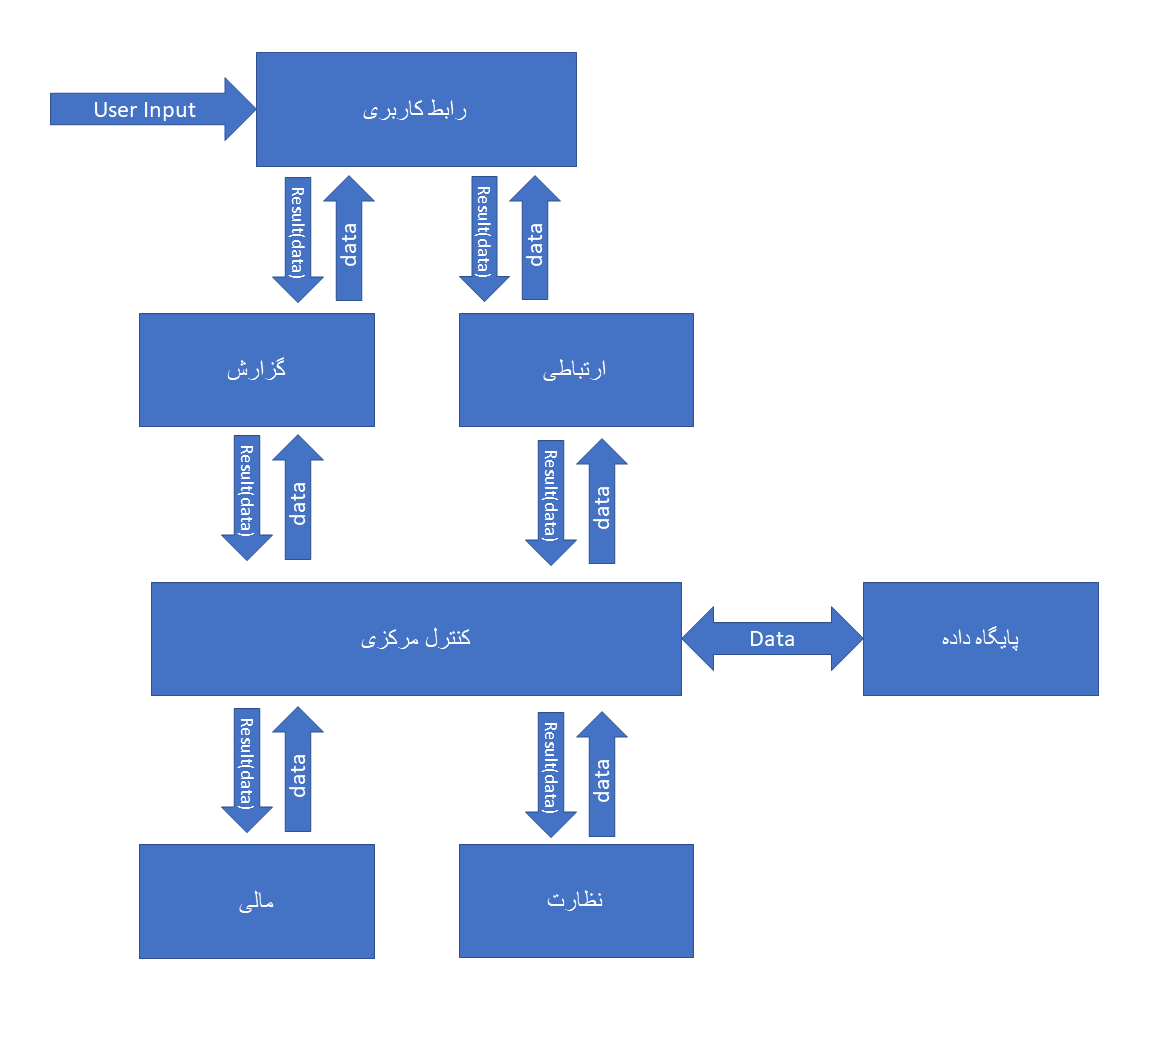
\includegraphics[height=13.5cm, width=16cm]{Chapter6.png}
			\caption{معماری سیستم ساهک}
		\end{center}
	\end{figure}
	
	\section{استفاده از یک سبک معماری}
	از آنجا که وظیفه اصلی سیستم تعامل با کاربر است، معماری آن نوعی معماری تعاملی است. وجود یک بخش
	سخت‌افزاری باعث تلفیق نوعی معماری رویداد-رانده با معماری چند لایه شده است.
	
	\section{اعمال قوانین طراحی نرم افزار}
	\subsection{طراحی برای تغییر}
	از آن جا که برای پاسخگویی به تغییرات در محیط کسب و کار، ارتقای کارایی و ... تغییر در سیستم امری ناگزیر است،
	ساهک به صورتی طراحی شده که تغییر در هر یک از اجزای آن به صورت مجزا و با صرف کمترین میزان وقت و هزینه
	امکان‌پذیر باشد. هدف از این طراحی تسهیل تغییرات قابل پیش‌بینی است.
	
	\subsection{جداسازی دغدغه ها}
	تمرکز هم‌زمان بر همه‌ی جوانب سیستم پارکینگ امری دشوار و هزینه بر است در نتیجه با توجه به قانون جداسازی
	دغدغه‌ها تلاش کردیم نیازمندی‌ها و زیرسیستم‌ها را هر یک در محدوده‌ی عملکرد خود به صورت جداگانه مورد بررسی و
	بحث قرار دهیم و در طراحی معماری مسئولیت های مربوط به دغدغه های مختلف را به زیرسیستم های آن ها اختصاص
	دهیم.
	
	\subsection{پنهان سازی اطلاعات}
	برای کاهش تبعات ناشی از تغییرات داده ساختارها در پایگاه داده و پیاده سازی توابع، معماری سیستم ما به گونه ای طراحی شده که جزئیات پیاده‌سازی و سازمان‌دهی پیمایش‌داده ساختارهای بخش‌های مختلف را از دید بقیه سیستم پنهان می‌کند. برای مثال واحد کنترل برقرار کننده ارتباط بین زیرسیستم‌های مختلف است و از نحوه ی پیاده‌سازی هر یک از زیر سیستم ها حفاظت می‌کند.
	
	\subsection{چسبندگی زیاد}
	\indent
	مولفه و کلاس‌های هر یک از زیرسیستم‌های موجود ارتباط زیادی با مسئولیت اصلی زیرسیستم‌های مرتبط دارند. برای مثال وظایف بخش های رهگیری، دوربین ها و سنسورها ارتباط نزدیکی با هم و مسئولیت اصلی گزارش را دارند.
	
	\subsection{جفت شدگی کم}
	در ساهک تلاش شده تا هر یک از زیرسیستم‌ها کمترین میزان وابستگی و تاثیر را بر دیگر زیرسیستم‌ها داشته باشند، به گونه ای که تغییر در هر یک از این زیرسیستم ها باعث بروز مشکلات عدیده در زیرسیستم دیگر نشود. برای مثال بخش نظارت بر پارکینگ از بخش محاسبه جریمه جدا شده و وابستگی به یکدیگر ندارند.
	
	\section{جمع بندی}
	برای طراحی معماری سیستم، با توجه به اهداف معماری و عملکرد هر واحد از سیستم، نوع معماری هر واحد را مشخص کردیم. سپس با در نظر گرفتن ارتباط بین آنها واسط‌های سیستم و نوع معماری کلی سیستم را تعیین کردیم. در طراحی معماری سعی شده که تا جای ممکن قوانین طراحی نرم افزار رعایت شود.
	
	
\chapter{مورد کاربرد}
\section{نمودار مورد کاربردها}
\begin{figure}[h]
	\begin{center}
		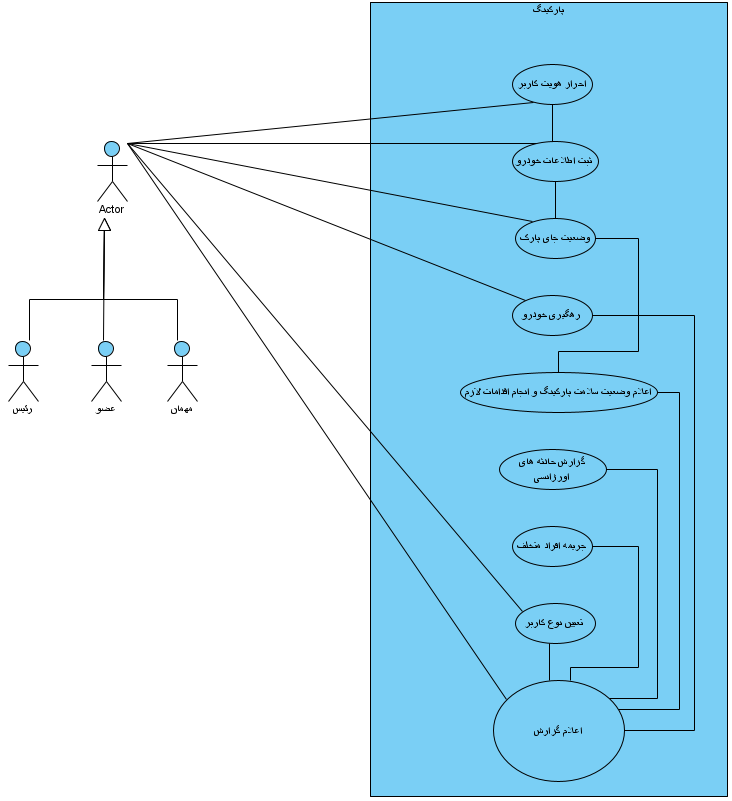
\includegraphics[height=10.9cm, width=13cm]{Use_Case_Diagram.png}
		\caption{نمودار مورد کاربردها}
	\end{center}
\end{figure}
\section{مورد کاربردهای سطح بالا}
\noindent
9 مورد از موردکاربردهای سیستم ساهک در ادامه اشاره شده است:\\

\lr{\textbf{-}} \hspace{5 mm} \lr{UC1} احراز هویت کاربر

\hspace{8 mm}	اولویت: 1
	
\hspace{8 mm}	کنشگر: کاربر، سیستم
	
\hspace{8 mm}	نیازمندی: \lr{R14, R09, R03, R01}
	
\hspace{16 mm}	\lr{TUCBW}: کاربر کارت را بر روی کارتخوان قرار می‌دهد.
	
\hspace{16 mm}	\lr{TUCEW}: کاربر پس از تایید احراز هویت کارت را برمی‌دارد.\\


\lr{\textbf{-}} \hspace{5 mm} \lr{UC2} ثبت اطلاعات خودرو

\hspace{8 mm}	اولویت: 1

\hspace{8 mm}	کنشگر: سیستم، کاربر

\hspace{8 mm}	نیازمندی: \lr{R14, R09, R08, R06, R02}

\hspace{16 mm}	\lr{TUCBW}: احراز هویت کاربر به وسیله‌ی کارت کاربر موفقیت آمیز بوده است.

\hspace{16 mm}	\lr{TUCEW}: سیستم کاربر را به جای پارک راهنمایی می‌کند.\\


\lr{\textbf{-}} \hspace{5 mm} \lr{UC3} وضعیت جای پارگ

\hspace{8 mm}	اولویت: 2

\hspace{8 mm}	کنشگر: سیستم

\hspace{8 mm}	نیازمندی: \lr{R09, R05, R04}

\hspace{16 mm}	\lr{TUCBW}: سنسورها متداولا وضعیت جای پارک را بررسی می‌کنند.

\hspace{16 mm}	\lr{TUCEW}: وضعیت جای پارک ها درمانیتور نشان داده می‌شود.\\


\lr{\textbf{-}} \hspace{5 mm} \lr{UC4} رهگیری خودرو

\hspace{8 mm}	اولویت: 3

\hspace{8 mm}	کنشگر: سیستم، کاربر

\hspace{8 mm}	نیازمندی: \lr{R09, R07}

\hspace{16 mm}	\lr{TUCBW}: کاربر شماره پلاک را مشخص می‌کند.

\hspace{16 mm}	\lr{TUCEW}: سیستم خودرو را نشان می‌دهد.\\


\lr{\textbf{-}} \hspace{5 mm} \lr{UC5} اعلام وضعیت سلامت پارکینگ و انجام اقدامات لازم

\hspace{8 mm}	اولویت: 3

\hspace{8 mm}	کنشگر: سیستم

\hspace{8 mm}	نیازمندی: \lr{R13, R11, R10}

\hspace{16 mm}	\lr{TUCBW}: وضعیت پارکینگ بررسی می‌شود.

\hspace{16 mm}	\lr{TUCEW}: هنگام آتش سوزی سیستم های اطفای حریق فعال می‌شود.\\\\


\lr{\textbf{-}} \hspace{5 mm} \lr{UC6} گزارش حادثه های اورژانسی

\hspace{8 mm}	اولویت: 3

\hspace{8 mm}	کنشگر: سیستم

\hspace{8 mm}	نیازمندی: \lr{R12}

\hspace{16 mm}	\lr{TUCBW}: سیستم باید حوادث را شناسایی کند.

\hspace{16 mm}	\lr{TUCEW}: در صورت وقوع حادثه با ارگان های مربوطه تماس حاصل کند.\\


\lr{\textbf{-}} \hspace{5 mm} \lr{UC7} جریمه افراد متخلف

\hspace{8 mm}	اولویت: 4

\hspace{8 mm}	کنشگر: سیستم، کاربر

\hspace{8 mm}	نیازمندی: \lr{R16, R15}

\hspace{16 mm}	\lr{TUCBW}: کاربر تخلفی انجام می‌دهد.

\hspace{16 mm}	\lr{TUCEW}: کاربر نسبت به گزارش موردنظر اقدامات لازم را انجام می‌دهد.\\


\lr{\textbf{-}} \hspace{5 mm} \lr{UC8} تعیین نوع کاربر

\hspace{8 mm}	اولویت: 1

\hspace{8 mm}	کنشگر: سیستم، کاربر

\hspace{8 mm}	نیازمندی: \lr{R17}

\hspace{16 mm}	\lr{TUCBW}: سیستم نوع کاربر را تعیین می‌کند.

\hspace{16 mm}	\lr{TUCEW}: دسترسی های مجاز را برای کاربر فعال می‌کند.\\


\lr{\textbf{-}} \hspace{5 mm} \lr{UC9} اعلام گزارش

\hspace{8 mm}	اولویت: 4

\hspace{8 mm}	کنشگر: سیستم، کاربر

\hspace{8 mm}	نیازمندی: \lr{R18, R19}

\hspace{16 mm}	\lr{TUCBW}: کاربر گزارشات را ثبت می‌نماید.

\hspace{16 mm}	\lr{TUCEW}: کاربر گزارش مربوطه را دیده و اقدامات لازم را انجام می‌دهد.
\vspace{7 cm} 

	\section{ماتریس ردیابی نیازمندی - مورد کاربرد}
		\begin{table}[h]
		\begin{center}
			\begin{tabular}{|>{\columncolor{blue!40!white}}c|c|c|c|c|c|c|c|c|c|c|}
				\hline
				\rowcolor{blue!40!white}
				\textbf{نیازمندی} & \textbf{اولویت} & \textbf{\lr{UC1}} & \textbf{\lr{UC2}} & \textbf{\lr{UC3}} & \textbf{\lr{UC4}} & \textbf{\lr{UC5}} & \textbf{\lr{UC6}} &
				\textbf{\lr{UC7}} & \textbf{\lr{UC8}} & \textbf{\lr{UC9}} \\
				\hline
				\lr{R01} & 1 & * & & & & & & & &\\
				\hline
				\lr{R02} & 1 & & * & & & & & & &\\
				\hline
				\lr{R03} & 1 & * & * & & & & & & &\\
				\hline
				\lr{R04} & 2 & & & * & & & & & &\\
				\hline
				\lr{R05} & 2 & & & * & & & & & &\\
				\hline
				\lr{R06} & 1 & & * & & & & & & &\\
				\hline
				\lr{R07} & 2 & & & & * & & & & &\\
				\hline
				\lr{R08} & 2 & & * & & & & & & &\\
				\hline
				\lr{R09} & 1 & * & * & * & * & & & & &\\
				\hline
				\lr{R10} & 2 & & & & & * & & & &\\
				\hline
				\lr{R11} & 3 & & & & & * & & & &\\
				\hline
				\lr{R12} & 3 & & & & & & * & & &\\
				\hline
				\lr{R13} & 2 & & & & & * & & & &\\
				\hline
				\lr{R14} & 1 & * & * & & & & & & &\\
				\hline
				\lr{R15} & 3 & & & & & & & * & &\\
				\hline
				\lr{R16} & 4 & & & & &  & & * & &\\
				\hline
				\lr{R17} & 1 & & & & & & & & * &\\
				\hline
				\lr{R18} & 5 & & & & & & & & & *\\
				\hline
				\lr{R19} & 5 & & & & & & & & & *\\
				\hline
				\multicolumn{2}{|c|}{\parbox[c]{3cm}{\cellcolor{blue!40!white}اولویت های مورد\\کاربردها}}&1&1&2&3&3&3&4&1&4\\
				\hline
			\end{tabular}
		\end{center}
		\caption{ماتریس ردیابی - موردکاربرد}
	\end{table}
\vspace{5cm}
\section{موردکاربردهای گسترده}
در ادامه به برخی از موردکاربردهای گسترده اشاره شده است.\\

\lr{UC1} احراز هویت کاربر

\begin{table}[h]
	\begin{center}
		\resizebox{\textwidth}{!}{
		\begin{tabular}{|p{8cm}|p{8cm}|}
			\rowcolor{blue!40!white}
				\textbf{\textcolor{white}{کنشگر: کاربر}} & \textbf{\textcolor{white}{سیستم: ساهک}} \\
				\rowcolor{black!10}
				 & 0. سیستم از کاربر میخواهد کارت خود را بر روی کارتخوان بگذارد.\\
				 \hline
				1. \lr{TUCBW}: کاربر کارت را بر روی کارتخوان قرار میدهد. &				
				\parbox{8cm}{2. سیستم هویت کاربر را تشخیص می‌دهدودرصورت صحت اطلاعات اجازه‌ی ورود می‌دهدو در هنگام خروج درصورت عدم تطابق اطلاعات کاربر با پایگاه داده موجود مورد را گزارش و مانع از خروج کاربر می‌شود. همچنین زمان ورود کاربر ذخیره می‌شود. سپس سیستم وضعیت کاربر را روی مانیتور نشان می‌دهد.}\\
				\hline
				\rowcolor{black!10}
				3. 	\lr{TUCEW}: کاربر پس از تایید احراز هویت کارت را برمی‌دارد. & \\
				\hline
		\end{tabular}
	}
	\end{center}
\caption{موردکاربرد گسترده احراز هویت کاربر}
\end{table}
\vspace{0.5cm}

\lr{UC 2} ثبت اطلاعات خودرو
\begin{table}[h]
	\begin{center}
		\resizebox{\textwidth}{!}{
			\begin{tabular}{|p{9cm}|p{9cm}|}
				\rowcolor{blue!40!white}
				\textbf{\textcolor{white}{کنشگر: کاربر}} & \textbf{\textcolor{white}{سیستم: ساهک}} \\
				\rowcolor{black!10}
				1. \lr{TUCBW}: کاربر درخواست ورود به پارکینگ را به سیستم می‌فرستد.
				&  2. سیستم برای شناسایی مکان‌های پارک موجود درخواستی به پارکینگ می‌فرستد. سپس پیامی برای کاربر ارسال می‌کند.\\			
				\hline
				3. 	\lr{TUCEW}: کاربر با توجه به نوع پیام، عملیات لازم را انجام می‌دهد.& \\
				\hline
			\end{tabular}
		}
	\end{center}
	\caption{مورد کاربر گسترده ثبت اطلاعات خودرو}
\end{table}

\vspace{0.5cm}

\lr{UC 4} رهگیری خودرو
\begin{table}[h]
	\begin{center}
		\resizebox{\textwidth}{!}{
			\begin{tabular}{|p{8cm}|p{8cm}|}
				\rowcolor{blue!40!white}
				\textbf{\textcolor{white}{کنشگر: کاربر}} & \textbf{\textcolor{white}{سیستم: ساهک}} \\
				\rowcolor{black!10}
				1. کاربر وارد اپلیکیشن می‌شود. &				
				2. سیستم شماره پلاک خودرو را درخواست می‌کند.\\
				\hline
				3. 	\lr{TUCEW}: کاربر شماره پلاک را به سیستم می‌فرستد. & 
				4. سیستم خودرو را نشان می‌دهد.\\
				\hline
				\rowcolor{black!10}
				5. \lr{TUCEW}: کاربر خودرو را دیده و عملیات لازم را انجام می‌دهد. & \\
				\hline
			\end{tabular}
		}
	\end{center}
	\caption{مورد کاربر گسترده رهگیری خودرو}
\end{table}

\vspace{2cm}
\lr{UC 7} جریمه افراد متخلف
\begin{table}[h]
	\begin{center}
		\resizebox{\textwidth}{!}{
			\begin{tabular}{|p{8cm}|p{8cm}|}
				\rowcolor{blue!40!white}
				\textbf{\textcolor{white}{کنشگر: کاربر}} & \textbf{\textcolor{white}{سیستم: ساهک}} \\
				\rowcolor{black!10}
				 1. \lr{TUCBW}: کاربر تخلفی انجام می‌دهد.
				 & 2. سیستم تخلف را شناسایی و کاربر را جریمه می‌کند. \\
				\hline			
		3. کاربر جریمه را می‌بیند. & 
		4. 	سیستم جرایم را پس از مدتی بررسی می‌کند و درصورت عدم پرداخت توسط کاربر، برای کاربر یک گزارش می‌فرستد.\\
				\hline
				\rowcolor{black!10}
				5. \lr{TUCEW}: کاربر نسبت به گزارش موردنظر اقدامات لازم را انجام می‌دهد. & \\
				\hline
			\end{tabular}
		}
	\end{center}
	\caption{مورد کاربر گسترده جریمه افراد متخلف}
\end{table}

\vspace{0.5cm}

\lr{UC 9} اعلام گزارش
\begin{table}[h]
	\begin{center}
		\resizebox{\textwidth}{!}{
			\begin{tabular}{|p{8cm}|p{8cm}|}
				\rowcolor{blue!40!white}
				\textbf{\textcolor{white}{کنشگر: کاربر}} & \textbf{\textcolor{white}{سیستم: ساهک}} \\
				\rowcolor{black!10}
				 &	0.	سیستم گزارشات خود را ثبت می‌نماید.\\
				 \hline
				1. \lr{TUCBW}: کاربر گزارشات را ثبت می‌نماید. & 
			2. سیستم گزارشات  را جمع بندی و در اپلیکیشن قرار می‌دهد. \\
				\hline
				\rowcolor{black!10}
				3. \lr{TUCEW}: کاربر گزارش مربوطه را دیده و اقدامات لازم را انجام می‌دهد. & \\
				\hline
			\end{tabular}
		}
	\end{center}
	\caption{مورد کاربر گسترده اعلام گزارش}
\end{table}
\vspace{10cm}
\section{سناریوها، جدول سناریوهاونمودارهای توالی موردکاربرها}
در ادامه به سناریوها، جدول سناریو و نمودارهای توالی بعضی مورد کاربردها اشاره شده است.\\\\
\textbf{\lr{UC1 -} احراز هویت کاربر}\\

\hspace{-1cm} 1. کاربر کارت را بر روی کارتخوان قرار میدهد.\vspace{2mm}

\noindent 2.1: سیستم اطلاعات کارت را خوانده و برای \lr{DB manager} می‌فرستد.\vspace{4mm}

\noindent 2.2: \lr{DB manager} اطلاعات دریافت شده را با اطلاعات موجود درخود تطابق می‌دهد.\vspace{4mm}

2.2.1: اگر اطلاعات دریافت شده با اطلاعات موجود در \lr{DB manager} تطابق داشت،\vspace{4mm}

\hspace{1cm} 2.2.1.1: اگر کاربر جریمه‌ای پرداخت نشده داشته باشد،\vspace{4mm}

\hspace{2cm} 2.2.1.1.1: از خروج کاربر ممانعت می‌شود.\vspace{4mm}

\hspace{1cm} 2.2.1.2: درغیر اینصورت،\vspace{4mm}

\hspace{2cm} 2.2.1.2.1: زمان ورود یا خروج کاربر را در \lr{DB manager} ذخیره می‌کند.\vspace{4mm}

2.2.2: درغیر اینصورت،\vspace{4mm}

\hspace{1cm} 2.2.2.1: مورد گزارش شده و مانع از ورود یا خروج کاربر می‌شود.\vspace{4mm}

\noindent 2.3: اطلاعات کاربر بر روی مانیتور نمایش داده می‌شود.\\\\


\begin{table}[h]
	\begin{center}
		\resizebox{\textwidth}{!}{
			\begin{tabular}{|c|c|c|c|c|}
				\rowcolor{blue!40!white}
				\textbf{\textcolor{white}{\#}} & \textbf{\textcolor{white}{فاعل}} & \textbf{\textcolor{white}{کنش فاعل}} & 
				\textbf{\textcolor{white}{دیگرداده‌ها/اشیا}} & \textbf{\textcolor{white}{شیئی که کنش روی آن انجام می‌شود}} \\
				
				\rowcolor{black!10}
				1 & کاربر & قرار می‌دهد & کارت & کارتخوان\\
				\hline
				
	2.1 & سیستم & می‌فرستد & اطلاعات کارت & \lr{DB manager}\\
				\hline
	
				\rowcolor{black!10}
				2.2 & \lr{DB manager} & تطابق اطلاعات & اطلاعات دریافتی & \lr{DB manager} \\
				\hline
	
				2.2.1 & \multicolumn{4}{|c|}{اگر اطلاعات دریافت شده با اطلاعات موجود در \lr{DB manager} تطابق داشت،} \\
				\hline
	
				\rowcolor{black!10}		
				2.2.1.1 & \multicolumn{4}{|c|}{اگر کاربر جریمه‌ای پرداخت نشده داشته باشد،} \\
				\hline
				
				2.2.1.1.1 & \lr{DB manager} & می‌فرستد & ممانعت از خروج & سیستم \\
				\hline
				
				\rowcolor{black!10}
				2.2.1.2 & \multicolumn{4}{|c|}{در غیر اینصورت،} \\
				\hline
				
				2.2.1.1 & \lr{DB manager} & ذخیره می‌کند & زمان ورود یا خروج & \lr{DB manager} \\
				\hline
				
				\rowcolor{black!10}
				2.2.2 & \multicolumn{4}{|c|}{در غیر اینصورت،} \\
				\hline
				
				2.2.2.1 & \lr{DB manager} & می‌فرستد & گزارش و مجوز ورود یا خروج & سیستم \\
				\hline
				
				\rowcolor{black!10}
	2.3 & سیستم & نمایش داده می‌شود & اطلاعات کاربر & مانیتور \\
			\hline
			\end{tabular}
		}
	\end{center}
	\caption{سناریو موردکاربرد احراز هویت کاربر}
\end{table}

\begin{figure}
	\begin{center}
		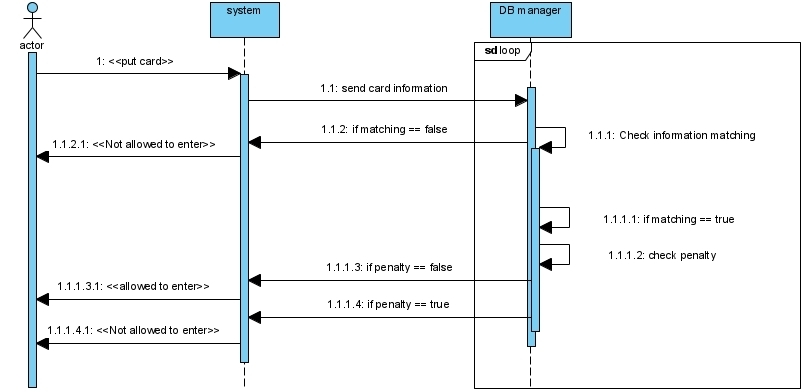
\includegraphics[height=10cm, width=15cm]{UC1 - Copy.jpg}
		\caption{نمودار توالی مورد کاربرد احراز هویت کاربر}
	\end{center}
\end{figure}

\vspace{6cm}
\noindent\textbf{\lr{UC2 -} ثبت اطلاعات خودرو}\\

\noindent 1:	کاربر درخواست ورود به پارکینگ را به سیستم می‌فرستد.\\

\noindent 2.1:  سیستم برای شناسایی مکان‌های پارک موجود درخواستی به پارکینگ می‌فرستد.\\

\noindent 2.2: پارکینگ مکان‌های پارک موجود در پارکینگ را شناسایی می‌کند.\\

\noindent 2.3: پارکینگ تعداد فضاهای خالی موجود درپارکینگ را به سیستم می‌فرستد.\\

2.3.1: اگر فضای خالی در پارکینگ موجود نبود، \\

\hspace{1cm} 2.3.1.1: اپلیکیشن پیام " در حال حاضر از ارائه خدمات به شما معذوریم " را به\\[-0.5cm]

\hspace{2.5cm}  کاربر نشان می‌دهد.

2.3.2: درغیر اینصورت،\\

\hspace{1cm} 2.3.2.1: سیستم شماره پلاک را به \lr{DB manager} می‌فرستد. \\

\hspace{1cm} 2.3.2.2: \lr{DB manager} شماره پلاک را در \lr{DB manage}r ثبت می‌کند.\\

\hspace{1cm} 2.3.2.3: \lr{DB manager} محل جای پارک را به اپلیکیشن می‌فرستد.\\

\hspace{1cm} 2.3.2.4: اپلیکیشن کاربر را به جای پارک راهنمایی می‌کند.\\


\begin{table}[h]
	\begin{center}
		\resizebox{\textwidth}{!}{
			\begin{tabular}{|c|c|c|c|c|}
				\rowcolor{blue!40!white}
				\textbf{\textcolor{white}{\#}} & \textbf{\textcolor{white}{فاعل}} & \textbf{\textcolor{white}{کنش فاعل}} & 
				\textbf{\textcolor{white}{دیگرداده‌ها/اشیا}} & \textbf{\textcolor{white}{شیئی که کنش روی آن انجام می‌شود}} \\
				
				\rowcolor{black!10}
				1 & کاربر & می‌فرستد & درخواست ورود & سیستم \\
				\hline
			
2.1 & سیستم &  می‌فرستد & درخواست شناسایی مکان های پارک موجود & پارکینگ\\
				\hline
			
				\rowcolor{black!10}	
	2.2 & پارکینگ & شناسایی می‌کند & مکان های پارک موجود & پارکینگ\\
				\hline
				
				
				2.3 & پارکینگ & می‌فرستد & تعداد فضاهای خالی & سیستم \\
				\hline
				
					\rowcolor{black!10}
				2.3.1 & \multicolumn{4}{|c|}{اگر فضای خالی در پارکینگ موجود نبود،} \\
				\hline
			
			2.3.1.1 & اپلیکیشن & نشان می‌دهد & پیام & کاربر \\
				\hline
			
				\rowcolor{black!10}
				2.3.2 & \multicolumn{4}{|c|}{در غیر اینصورت،} \\
				\hline
				
				
				2.3.2.1 & سیستم & می‌فرستد & شماره پلاک & \lr{DB manager}\\
				\hline
				
				\rowcolor{black!10}
				2.3.2.2 & \lr{DB manager} & ثبت می‌کند & شماره پلاک & \lr{DB manager} \\
				\hline
				
				2.3.2.3 & \lr{DB manager} & می‌فرستد & محل جای پارک & اپلیکیشن\\		\hline		
				
				\rowcolor{black!10}
			2.3.2.4 & اپلیکیشن & راهنمایی می‌کند & جای پارک & کاربر\\
				\hline
				
			\end{tabular}
		}
	\end{center}
	\caption{سناریو موردکاربرد ثبت اطلاعات خودرو}
\end{table}

\begin{figure}
	\begin{center}
		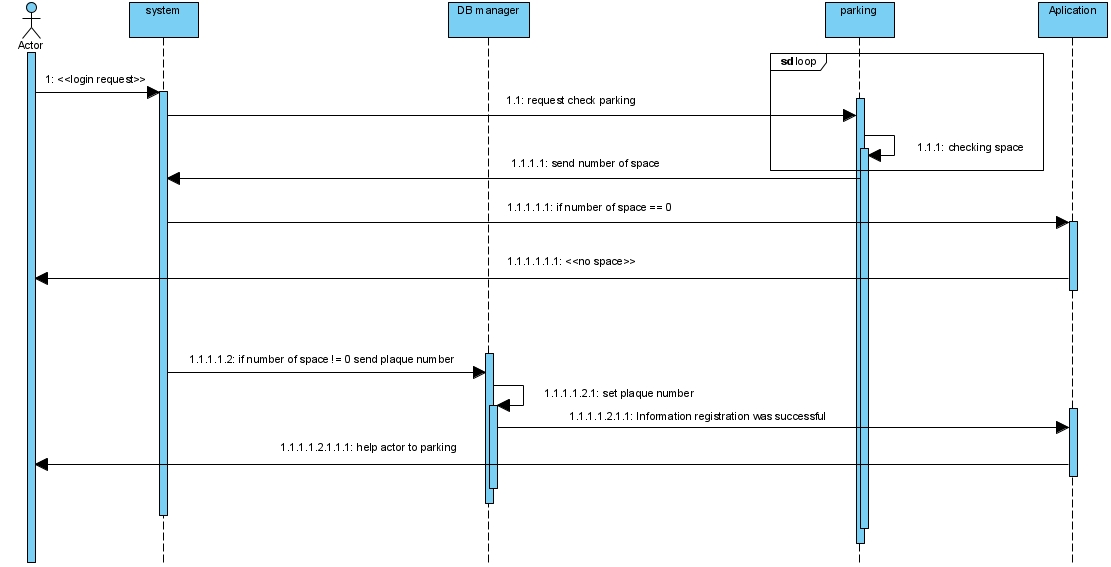
\includegraphics[height=10cm, width=15cm]{UC2.jpg}
		\caption{نمودار توالی مورد کاربرد ثبت اطلاعات خودرو}
	\end{center}
\end{figure}
\vspace{6cm}

\noindent\textbf{\lr{UC4 -} رهگیری خودرو}\\

\noindent 3.1: کاربر شماره پلاک را به سیستم می‌فرستد.\\

\noindent 3.2: سیستم شماره پلاک را برای \lr{DB manager} می‌فرستد.\\

\noindent 3.3: \lr{DB manager} شماره پلاک را در \lr{DB manager} جستجو می‌کند. \\

 3.3.1: اگر شماره پلاک در \lr{DB manager} موجود باشد، \\

\hspace{1cm} 3.3.1.1: \lr{DB manager} موقعیت خودرو را برای سیستم می‌فرستد.\\

\hspace{1cm} 3.3.1.2: سیستم نزدیکترین دوربین در پارکینگ را پیدا می‌کند.\\

\hspace{1cm} 3.3.1.3: پارکینگ تصاویر زنده را برای اپلیکیشن می‌فرستد.\\

\hspace{1cm} 3.2.1.4: اپلیکیشن تصاویر زنده را برای کاربر می‌فرستد.\\

3.3.2: درغیر اینصورت،\\

\hspace{1cm} 3.2.2.1: سیستم پیام "پلاک موردنظر یافت نشد" را برای اپلیکیشن می‌فرستد.\\

\hspace{1cm} 3.2.2.2: اپلیکیشن پیام موردنظر را به کاربر نشان می‌دهد. \\\\

\begin{table}[h]
	\begin{center}
		\resizebox{\textwidth}{!}{
			\begin{tabular}{|c|c|c|c|c|}
				\rowcolor{blue!40!white}
				\textbf{\textcolor{white}{\#}} & \textbf{\textcolor{white}{فاعل}} & \textbf{\textcolor{white}{کنش فاعل}} & 
				\textbf{\textcolor{white}{دیگرداده‌ها/اشیا}} & \textbf{\textcolor{white}{شیئی که کنش روی آن انجام می‌شود}} \\
				
				\rowcolor{black!10}
			3.1 & کاربر & می‌فرستد & شماره پلاک & سیستم \\
				\hline
				
	  3.2 & سیستم & می‌فرستد & شماره پلاک & \lr{DB manager} \\
				\hline
				
				\rowcolor{black!10}				
     			3.3 & \lr{DB manager} & جستجو می‌کند & شماره پلاک & \lr{DB manager}\\
				\hline
				

				3.3.1 & \multicolumn{4}{|c|}{اگر شماره پلاک در\lr{DB manager}موجود باشد،}\\
				\hline
				
				\rowcolor{black!10}
			3.3.1.1 & \lr{DB manager} & می‌فرستد & موقعیت خودرو & سیستم \\
			\hline
				
3.3.1.2 & سیستم & پیدامی‌کند & نزدیکترین دوربین & پارکینگ\\
				\hline
				
				\rowcolor{black!10}
	3.3.1.3 & پارکینگ & می‌فرستد & تصاویر زنده & اپلیکیشن \\
				\hline
								
	3.3.1.4 & اپلیکیشن & نشان می‌دهد & تصاویرزنده & کاربر \\
				\hline
				
				\rowcolor{black!10}
				3.3.2 & \multicolumn{4}{|c|}{در غیر اینصورت،} \\
				\hline
				
				3.3.2.1 & سیستم & می‌فرستد & پیام & اپلیکیشن \\
				\hline
								
				\rowcolor{black!10}
	    	3.2.2.2 & اپلیکیشن & نشان می‌دهد & پیام & کاربر \\
				\hline
				
			\end{tabular}
		}
	\end{center}
	\caption{سناریو موردکاربرد رهگیری خودرو}
\end{table}

\begin{figure}
	\begin{center}
		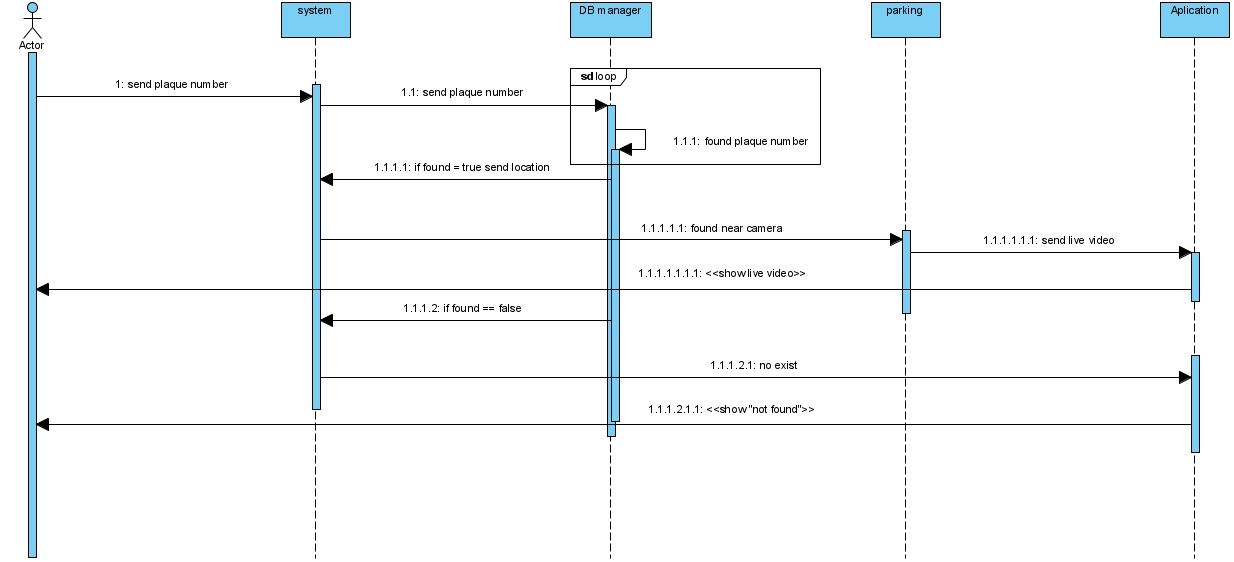
\includegraphics[height=10cm, width=15cm]{UC4.jpg}
		\caption{نمودار توالی مورد کاربرد رهگیری خودرو}
	\end{center}
\end{figure}

\chapter{نمودار کلاس طراحی}
\section{چگونگی نحوه رسم نمودار کلاس طراحی}
با توجه به 3 نمودار توالی رسم شده، ما کلاس های \lr{Actor}، \lr{System}، \lr{Parking}، \lr{DB manager} و \lr{Application} را استخراج کردیم.\\

با توجه به آنکه کاربر برای ورود باید کارت خود را برروی کارتخوان قرار دهد، پس کلاس \lr{Actor} دارای صفت‌های \lr{id} و \lr{card} و تابع \lr{Send_information()} و \lr{Send_requests()} را برای ارسال اطلاعات و ایجاد درخواست دارد.\\

کلاس \lr{System} اطلاعاتی را دریافت می‌کند و با توجه به اطلاعات دریافتی اقدامات لازم را انجام می‌دهد. بدین منظور دارای صفت \lr{information} و توابع \lr{Send_information()} و\\ \lr{Send_requesets()} و \lr{Find_camera()} می‌باشد.\\

کلاس \lr{Parking} دارای صفت های \lr{space}، \lr{location} و \lr{camera} به منظور کنترل فضای پارکینگ می‌باشد و این اطلاعات را با استفاده از توابع \lr{Send_information()} و \lr{Check_space()} به کلاس های \lr{System} و \lr{Application } می‌فرستد.\\

کلاس \lr{DB manager} دارای صفت های \lr{penalty}،\lr{ actor information} و \lr{plaque number} به منظور نگهداری اطلاعات کاربر یا خودرو و میزان جریمه می‌باشد. در این کلاس از توابع\\ \lr{Authentication()} برای احراز هویت کاربر، \lr{Check_penalty()} برای بررسی جریمه،\\ \lr{Save_ information()} برای ذخیره اطلاعات، \lr{Search()} برای جستجو در پایگاه داده و\\ \lr{Send_ information()} برای ارسال اطلاعات به \lr{System} و \lr{Application}استفاده شده است.\\

در کلاس \lr{Application}  از توابع \lr{Get_information()} برای دریافت اطلاعات،\\ \lr{Show_message() } برای نمایش پیامی متناسب با اطلاعات دریافت شده به کاربر، \lr{Help_actor() }برای راهنمایی کاربر و \lr{Show_live_video() }برای نشان دادن پارکینگ به کاربر از طریق دوربین‌ها استفاده شده است.\\

\vspace{-1cm}
\section{نمودار کلاس طراحی}
\begin{figure}[h]
	\begin{center}
		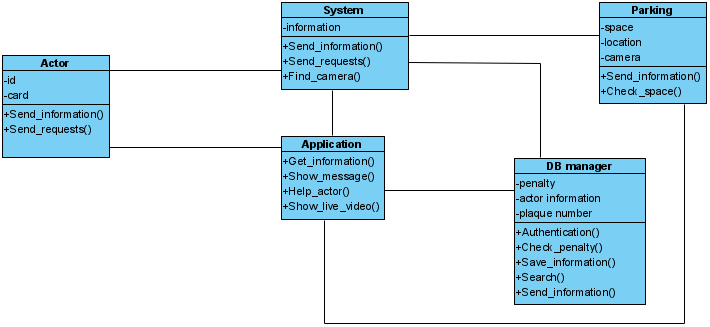
\includegraphics[height=6cm, width=14cm]{ClassDiagram.png}
		\caption{کلاس طراحی}
	\end{center}
\end{figure}
\section{دست آوردهای پروژه}
توانستیم در این پروژه صبر و بردباری خود را بالا برده و با انجام پروژه به روش اسکرام(مکالمات تلفنی روزانه و هفتگی) پروژه را به نحوه احسن به پایان رسانیم.

با تهیه سند نیازمندی ها و استخراج مورد کاربردها قلمروی سیستم خود را مشخص کردیم و در نهایت با طراحی
معماری و نمودار های توالی و نمودار دامنه کلاس دید دقیق و قطعی تری نسبت به عملکرد سیستم پیدا کردیم.

نحوه کار با نرم افزارهای \lr{Visual paradigm} و \lr{TeXstudio} در طی انجام پروژه آموختیم.

همچنین در طی انجام این پروژه آموختیم که برای انجام پروژه نیاز به حضور فیزیکی اعضا در کنار یکدیگر نیست و به روش مجازی هم می‌توان به سختی پروژه انجام داد.

در حین انجام این پروژه به دفعات زیاد با پروژه های عملی بازار کار روبرو شدیم و توانستیم از این درس و پروژه با مشکلات متعددی که همراه بود سربلند بیرون بیاییم.

\section{نرم افزارهای استفاده شده در پروژه}
\lr{Texstudio}

\lr{Microsoft Word}

\lr{Microsoft PowerPoint}

\lr{Visual Paradigm}
\end{document}
